\begin{figure}[h]
	%\centering
	\hspace{-0.25\linewidth}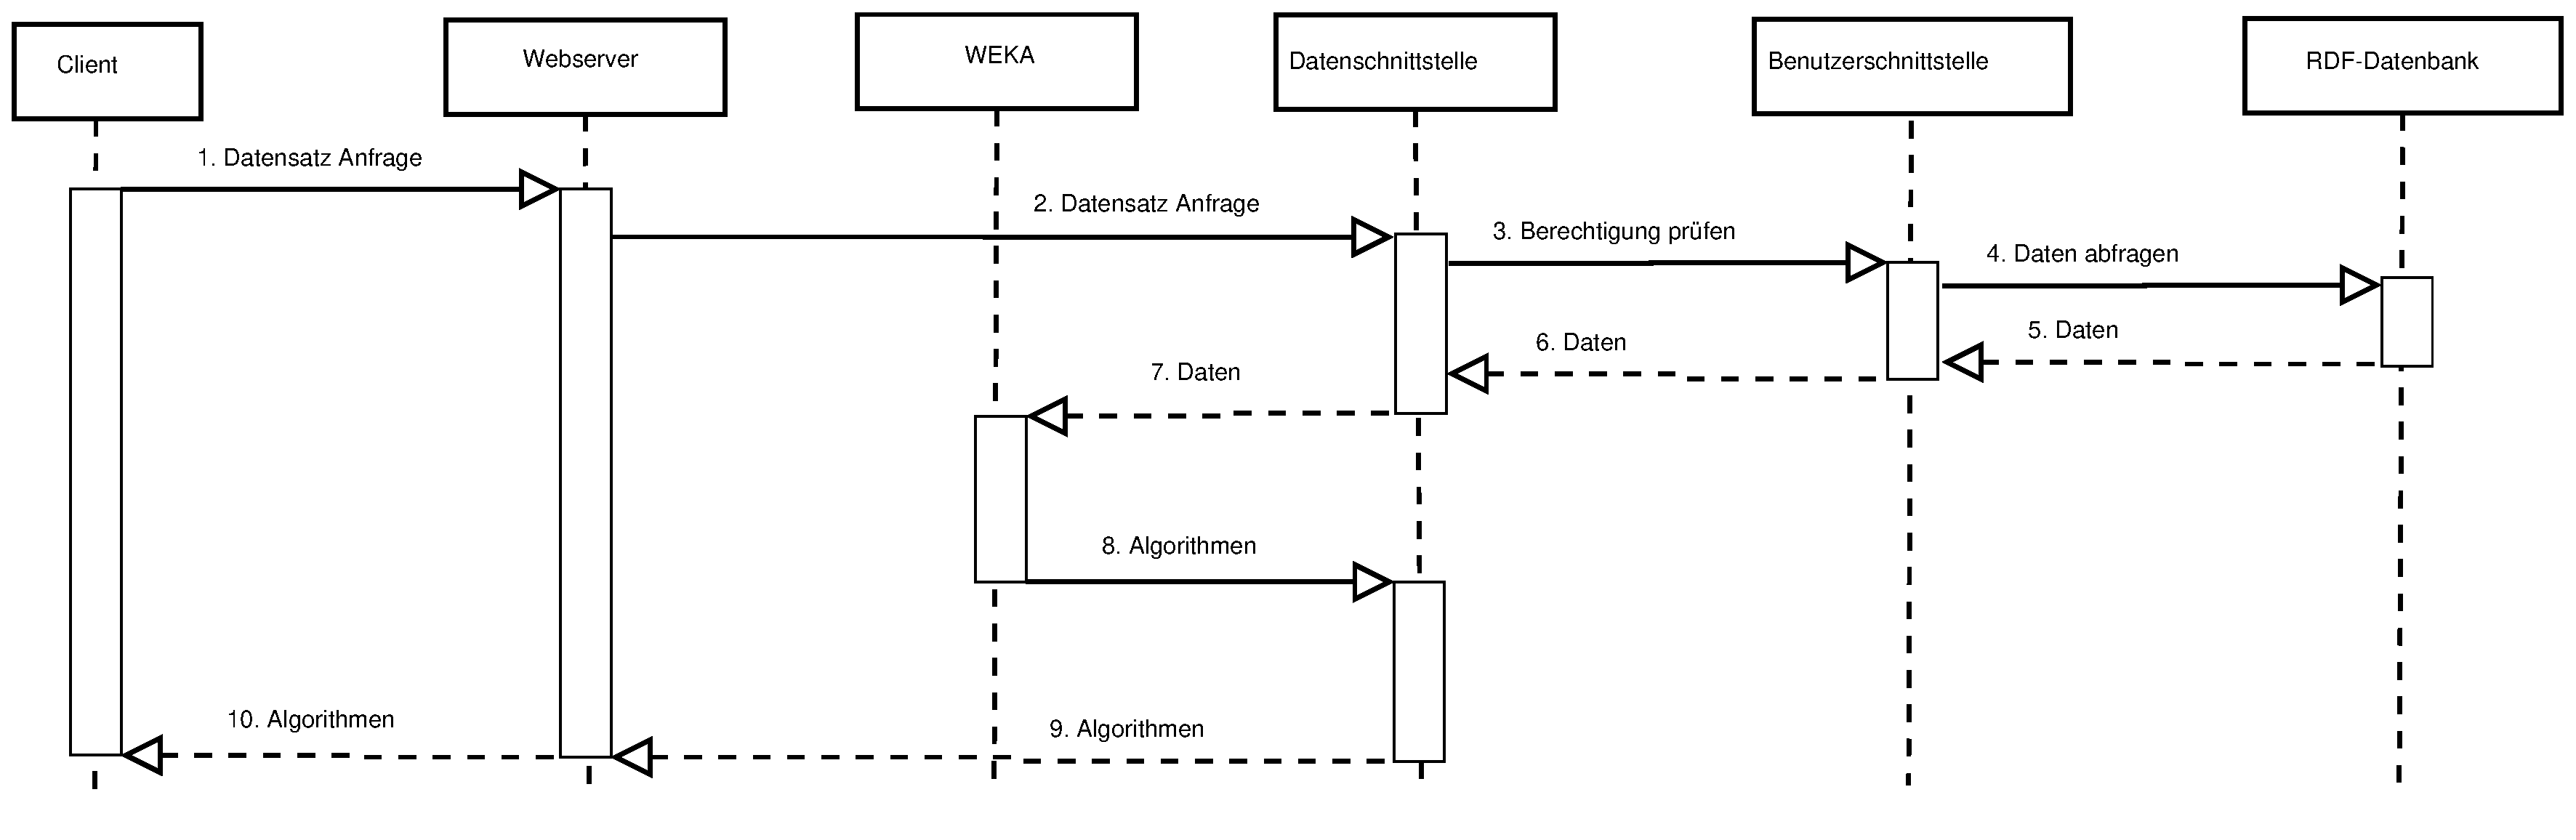
\includegraphics[width=1.5\linewidth]{Grafik/Diagramm/Szenarios/Berechnung}
	\caption[]{Auswahl eines Datensatzes}
\end{figure}
\noindent Um aus einem vorher hochgeladenen Datensatz ein Modell zu berechnen, muss der Nutzer diesen zuerst auswählen. Diese Aktion wird an den Webserver weitergeleitet, welcher wiederum eine Anfrage an die Datenschnittstelle sendet. Diese entnimmt den Daten der Anfrage wo sich der Datensatz befindet und sendet daraufhin eine Anfrage an die Benutzerschnittstelle, welche überprüft ob ein Zugriff auf die Daten durch den Nutzer erlaubt ist. Steht dem Zugriff auf die Daten keine Beschränkung entgegen, so leitet die Benutzerschnittstelle die Anfrage an die entsprechende Datenbank weiter. Diese gibt die angeforderten Daten über die Benutzerschnittstelle zurück an die Datenschnittstelle. Dort wird der Datensatz zur Analyse an das WEKA-Modul weitergeleitet, welches feststellt, welche der vorhandenen Algorithmen den Datensatz verarbeiten können. Diese Liste an Algorithmen wird wieder an die Datenschnittstelle zurückgegeben, welche wiederum die Daten an den Webserver weitergibt. Dieser gibt die Daten passend an den Client weiter, so dass diesem angezeigt werden kann, welche Algorithmen mit dem gewählten Datensatz verwendet werden können.\\

\begin{figure}[h]
	%\centering
	\hspace{-0.25\linewidth}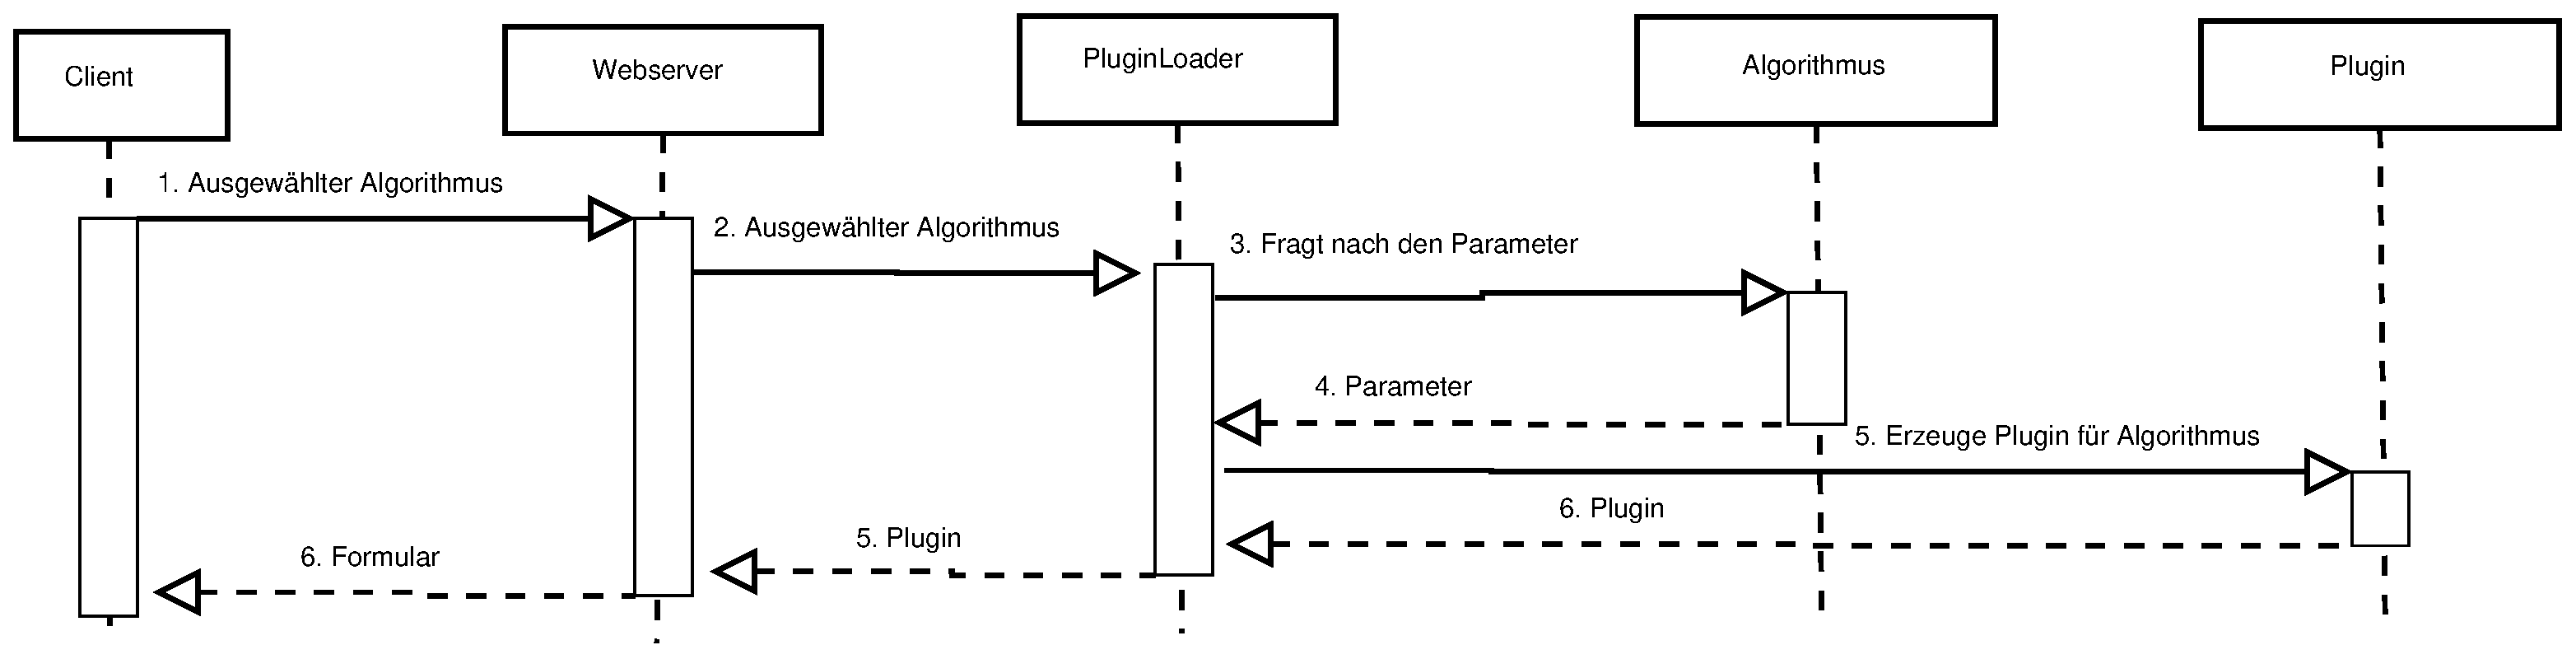
\includegraphics[width=1.5\linewidth]{Grafik/Diagramm/Szenarios/Berechnung2}
	\caption[]{Auswahl eines Algorithmus}
\end{figure}
\noindent Hat der Nutzer nun einen Algorithmus ausgewählt, so wird dieser an den Webserver weiter gegeben. Der fordert nun den PluginLoader auf ihm ein Plugin zur Erzeugung eines Formulars für diesen Algorithmus zu geben. Dafür fragt der PluginLoader den Algorithmus, nach den Parametern, die er zur Ausführung benötigt. Aus dieser Information erzeugt der PluginLoader nun ein Plugin für diesen Algorithmus, welcher dann wiederum über den PluginLoader an den Webserver weitergegeben wird. Dieser erzeugt nun mit der Hilfe des Plugins ein Formular mit den Parametern, welches er wiederum dem Client schickt.
\pagebreak
\begin{wrapfigure}{l}{0.4\textwidth}
	\vspace{-80pt}
	\begin{center}
		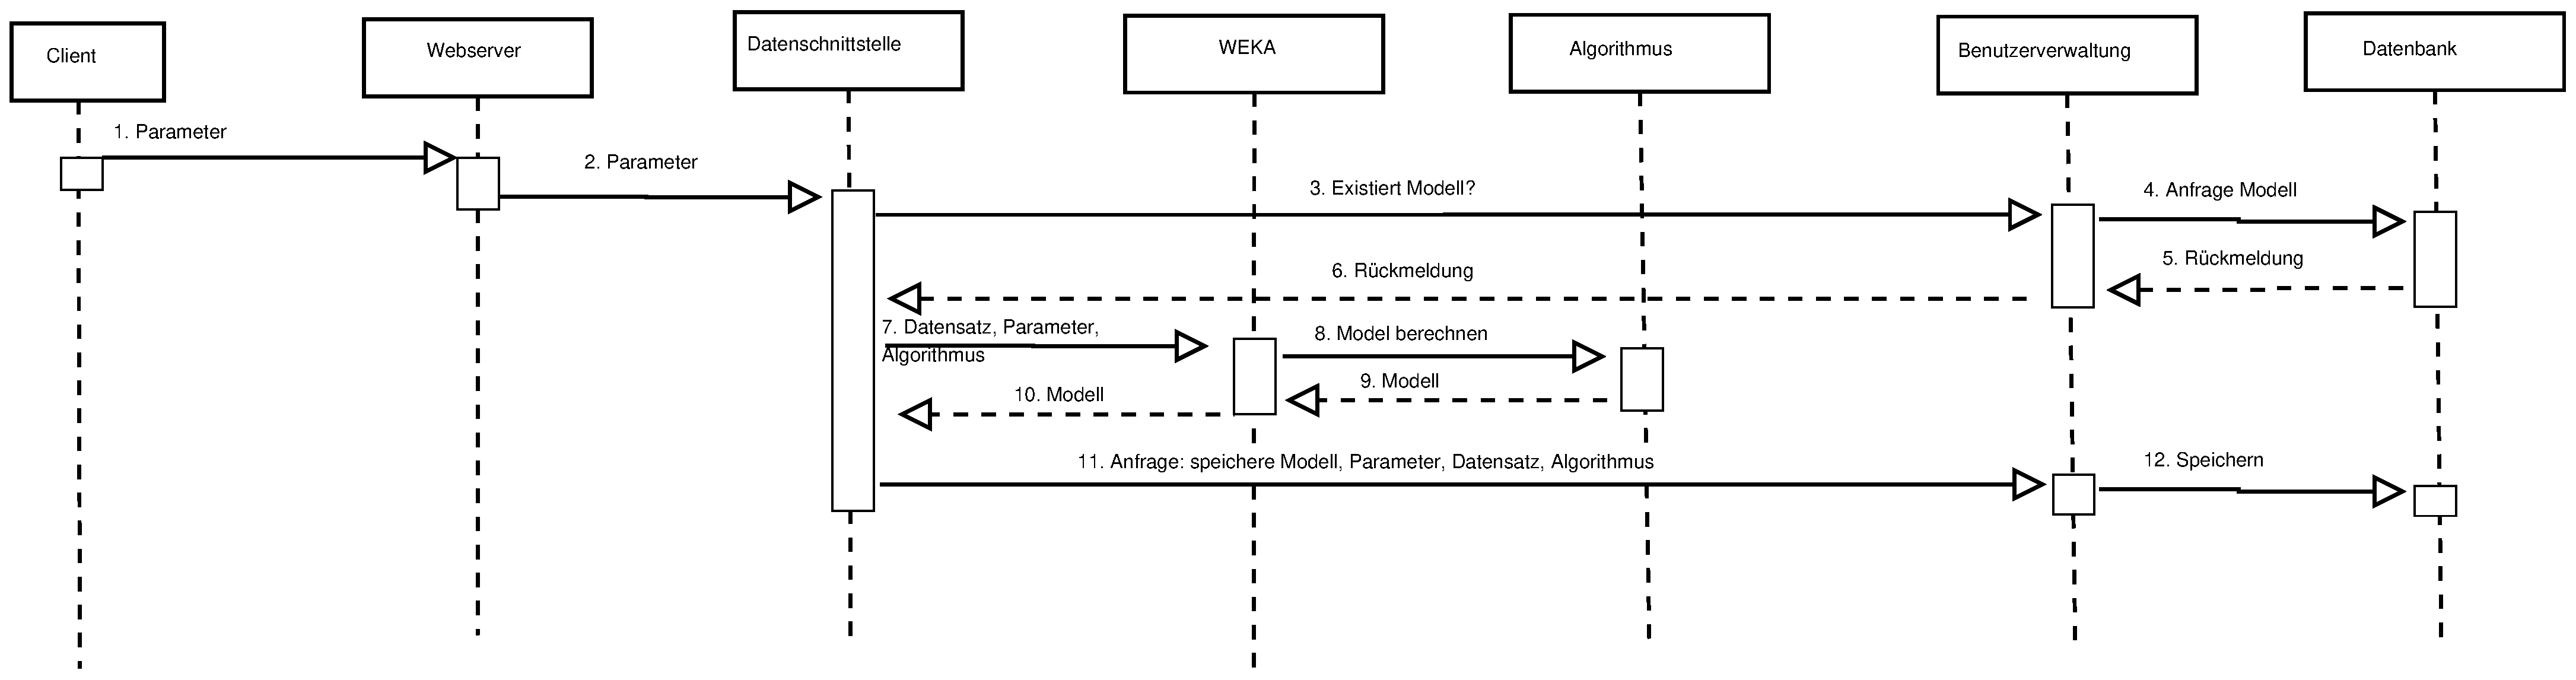
\includegraphics[width =1\textheight, angle=90 ]{Grafik/Diagramm/Szenarios/Berechnung3}
	\end{center}
	\vspace{-15pt}
	\caption[]{Berechnung eines Modells}
	\label{fig:Berechnung3}
	\vspace{-70pt}
\end{wrapfigure}\\
Wurden schließlich Datensatz, Algorithmus und Parameter gesetzt, werden diese über den Webserver an die Datenschnittstelle übergeben. Diese überprüft nun ob ein Modell für diese Kombination an Datensatz, Algorithmus und Parametern in der Datenbank existieren, die Benutzerverwaltung reglementiert dabei, welche Bereiche der Datenbank der Nutzer in seiner Rolle einsehen kann. Ob ein solches Modell existiert wird anschließend an die Datenschnittstelle weitergegeben. Existiert kein solchen Modell oder entscheidet sich der Nutzer dafür ein neues Modell zu erstellen, so übergibt die Datenschnittstelle die erforderlichen Daten an das WEKA-Modul. Dieses lässt nun von dem passenden Algorithmus das Modell berechnen und gibt dieses an die Datenschnittstelle zurück. Diese speichert nun das Modell mit den genutzten Daten in der Datenbank, da der Nutzer während der Berechnung nicht blockiert sein soll. Dieser kann anschließend zu einem beliebigen Zeitpunkt das Modell aus der Datenbank abrufen.